%\chapterauthor{Author Name}{Author Affiliation}
%\chapterauthor{Second Author}{Second Author Affiliation}
\chapter{Brief Introduction to Linux}

This chapter gives a brief introduction to Linux, including some of its key features and advantages/disadvantages comparing with other operating systems.

\section{Brief Introduction}

Linux is an operating system (OS). An OS is essentially a special piece of software running on a machine (computer, server, mobile devices, or other electrical devices capable and sophisticated enough to host an OS) that manages hardware resources of the system and provides services to the application software in the upper layer. An OS shall be able to
\begin{itemize}
  \item detect and prepare hardware;
  \item manage processes;
  \item manage memory;
  \item provide user interface and user authentication;
  \item manage file systems;
  \item provide programming tools for creating applications.
\end{itemize}

Linux has been overwhelmingly successful and adopted in many areas. For example, Android operating system for mobile phones is developed using Linux. Google Chrome is also backed by Linux. Many famous websites including Facebook are also running on Linux servers.

Some of the most favorable features of Linux (especially to large size enterprises) are as follows.
\begin{itemize}
  \item Clustering: multiple machines work together as a whole, and they appear to be a single machine to upper layer applications.
  \item Visualization: one machine hosts multiple applications, each of which thinking that it is running on a dedicated machine.
  \item Cloud computing: flexible resources management is achieved by running applications on clouds on virtual machines running Linux OS.
  \item Real-time computing: embedded Linux is implemented on micro-controllers or micro-computers for real-time edge control.
\end{itemize}

Linux differs from Microsoft Windows and MacOS in many ways, though they are all very good OSs. Among the three OSs, Linux is the only OS that is completely open-source (in the sense that all its code can be viewed and modified per requested) and can be flexibly customized by the users.

\section{A Short History of Linux}

The initial motivation of Linux is to create a UNIX-like operating system that can be freely distributed in the community.

Many modern OSs including MacOS and Linux are derived from UNIX. UNIX operating system was created by AT\&T in 1969 as a software development environment that AT\&T used internally. In 1973, UNIX was rewritten in C language, thus gaining useful features such as portability. Today, C is still the primary language used to create UNIX (and also Linux) kernels.

AT\&T, who originally owned UNIX, tried to make money from it. Back then AT\&T was restricted from selling computers as required by the government. Therefore, AT\&T decided to license UNIX source code to universities for a nominal fee. Researchers from universities started learning and improving UNIX, which speeded up the development of UNIX. In 1976, UNIX V6 became the first UNIX that was widely spread. UNIX V6 was developed at UC Berkeley and was named the Berkeley Software Distribution (BSD) of UNIX.

From then on, UNIX moved towards two separate directions: BSD continued forward in the ``open'' and ``share'' manner, while AT\&T started steering UNIX towards commercialization. By 1984 AT\&T was pretty ready to start selling commercialized UNIX, namely ``AT\&T: UNIX System Laboratories (USL)''. USL did not sell very well. As said, AT\&T could only sell the OS source code to other PC manufactures, but not the PC itself with UNIX pre-installed. For this reason the price for the source code had to be set high as it is targeted for PC manufactures, not for end users. This largely prevented an end user from procuring UNIX source code from AT\&T directly. The PC manufactures were in fact more successful than AT\&T just by selling UNIX based PC and workstations to the end users. Overall, although the community acknowledged that UNIX was useful, UNIX source code was extremely costly and was not popular among the end users.

In 1984, Richard Stallman started the GNU project as part of the Free Software Foundation. It is recursively named by phrase ``GNU is Not UNIX'', intended to become a recording of the entire UNIX that could be open and freely distributed. The community started to ``recreate'' UNIX based on the defined interface protocols published by AT\&T.

Linus Trovalds started creating his version of UNIX, i.e. Linux, in 1991. He managed to publish the first version of the Linux kernel on August 25, 1991, which only worked on a 386 processor. Later in October, Linux 0.0.2 was released with many parts of the code rewritten in C language, making it more suitable for cross-platform usage. This Linux kernel was the last and the most important piece of code to complete a UNIX-like system under GNU General Public License (GPL). It is so important that people call this operating system ``Linux OS'' instead of ``GNU OS'', although GNU is the host of the project and Linux kernel is just a part (the most important part) of it.

\section{Linux Distributions}

As casual Linux users, people do not want to understand and compile the Linux source code to use Linux. In response to this need, different Linux distributions have merged. They share the same Linux OS kernel but differ from each other in many ways such as software management tools and user interfaces.

Today, there are hundreds of Linux distributions in the community. The most famous two categories of distributions are as follows. Notice that although the source code of them are available in public as required by GPL license (GPL requires that any modified version of GPL licensed product shall also be made open-source with a GPL license, as long as the modification spreads in the community), some of the distributions may come with a ``subscription fee''. The subscription fee is not for the source code, but for the technical support, paid maintenance, and other services that convene the life of the users.
\begin{itemize}
  \item Red Hat Based Distributions
  \begin{itemize}
    \item Red Hat Enterprise Linux (RHEL)
    \item Fedora
    \item CentOS
  \end{itemize}
  \item Debian Based Distributions
  \begin{itemize}
    \item Debian
    \item Ubuntu
    \item Linux Mint
    \item Elementary OS
    \item Raspberry Pi OS
  \end{itemize}
\end{itemize}

Some of the main features of Red Hat based distributions are as follows. Red Hat created the Red Hat Package Manager (RPM) to manage the installation and upgrading of software. The RPM packaging contains not only the software files but also its metadata, including version tracking, the creator, the configuration files, etc. In the OS, a local RPM database is used to track all software on the machine. Anaconda installer simplifies the installation of Red Hat Linux, meantime leaving users enough flexibility for customization. Red Hat OS is integrated with simple graphical tools for device management (such as adding a printer), user management and other administration work.

Red Hat Enterprise Linux (RHEL) is a commercial, stable and well-supported OS that can host mission-critical applications for big business and governments. To use RHEL, customers buy subscriptions which allow them to deploy any version of RHEL as desired. Different levels of support are available depending on customers needs. Many add-on features, including cloud computing integration, are available for the customers.

CentOS is a ``recreation'' version of RHEL using freely available RHEL source code. In this sense, CentOS experience should be very similar with RHEL and it is free of charge, but the users will not enjoy the professional technical support from RHEL engineers.
Recently, Red Hat took over the development of CentOS project.

Fedora is a free, cutting-edge Linux distribution sponsored by Red Hat. It is less stable than RHEL, and plays as the ``testbed'' for Red Hat to interact with the community. From this perspective, Fedora is very similar to RHEL, just with more dynamics and uncertainties. Some functions, especially server related functions, will be tested on Fedora before implementation on RHEL.

Different from Red Hat based distributions that use RPM, Debian and Debian based distributions use Advanced Packaging Tool (APT) to manage software. ATP simplifies the process of managing software by automating the retrieval, configuration and installation of  software packages, either form pre-compiled files or by compiling source code. Among all Debian based distributions, Ubuntu is the most successful and popular one. Ubuntu has a variety of graphical tools and focuses on full-featured desktop system while still offering popular server packages. It has a very active community to support its development.

Ubuntu has larger software pool than Fedora. Ubuntu and its associated software usually have a longer ``lifespan'' than Fedora in the sense that Ubuntu is target for more stable use while Fedora is more of a ``testbed''. In this sense, Ubuntu is more for casual users and Fedora more for advanced users or developers, especially developers for RHEL.

\section{Linux Graphical Desktop}

Though not necessary for Linux, both Ubuntu and Fedora distributions (and many other Linux distributions) support graphical desktops. By default, both systems come with GNOME graphical desktop environment. There are other choice of graphical desktops, such as KDE, LXDE and Xfce desktops. GNOME and KDE are more for regular computers while LXDE and Xfce are light in size, thus more for low-power-demanding systems.

Figs. \ref{ch:bitl:fig:gnomedemo}, \ref{ch:bitl:fig:kdedemo}, \ref{ch:bitl:fig:lxdedemo} and \ref{ch:bitl:fig:xfcedemo} give the flavors of each desktop environment mentioned above. From the figures we can see that GNOME adopts a more Linux/MacOS style desktop environment, while KDE has a ``Windows 7'' style desktop. LXDE and Xfce are more simple in graphics presentations and they are more for embedded systems.

\begin{figure}
	\centering
	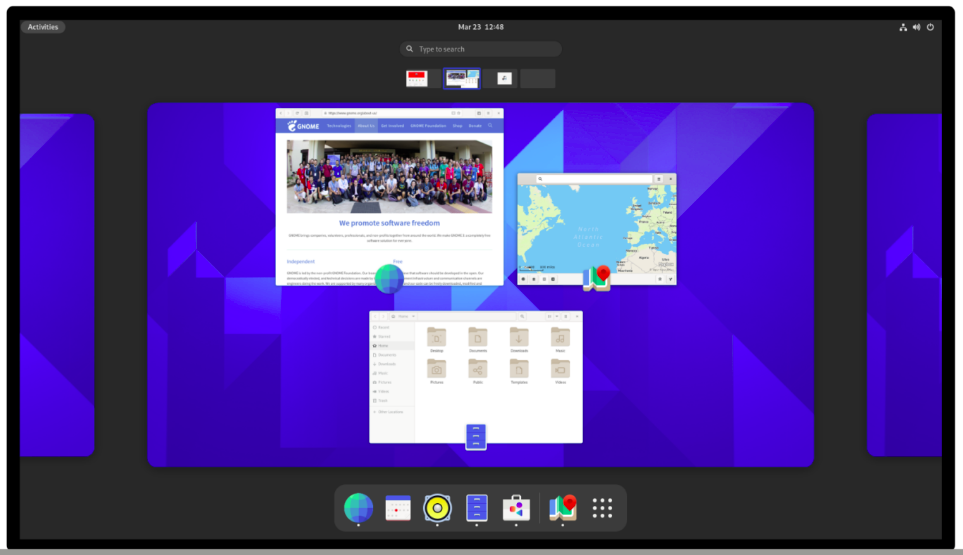
\includegraphics[width=250pt]{chapters/ch-brief-introduction-to-linux/figures/gnome_demo.png}
	\caption{GNOME desktop environment.} \label{ch:bitl:fig:gnomedemo}
\end{figure}

\begin{figure}
	\centering
	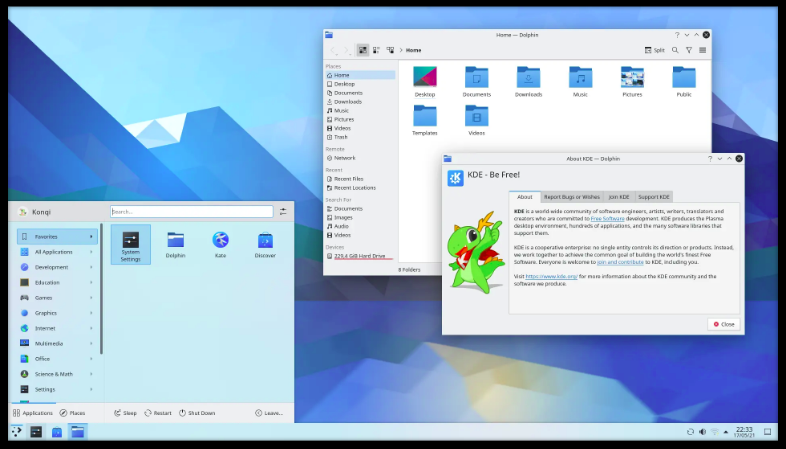
\includegraphics[width=250pt]{chapters/ch-brief-introduction-to-linux/figures/kde_demo.png}
	\caption{KDE desktop environment.} \label{ch:bitl:fig:kdedemo}
\end{figure}

\begin{figure}
	\centering
	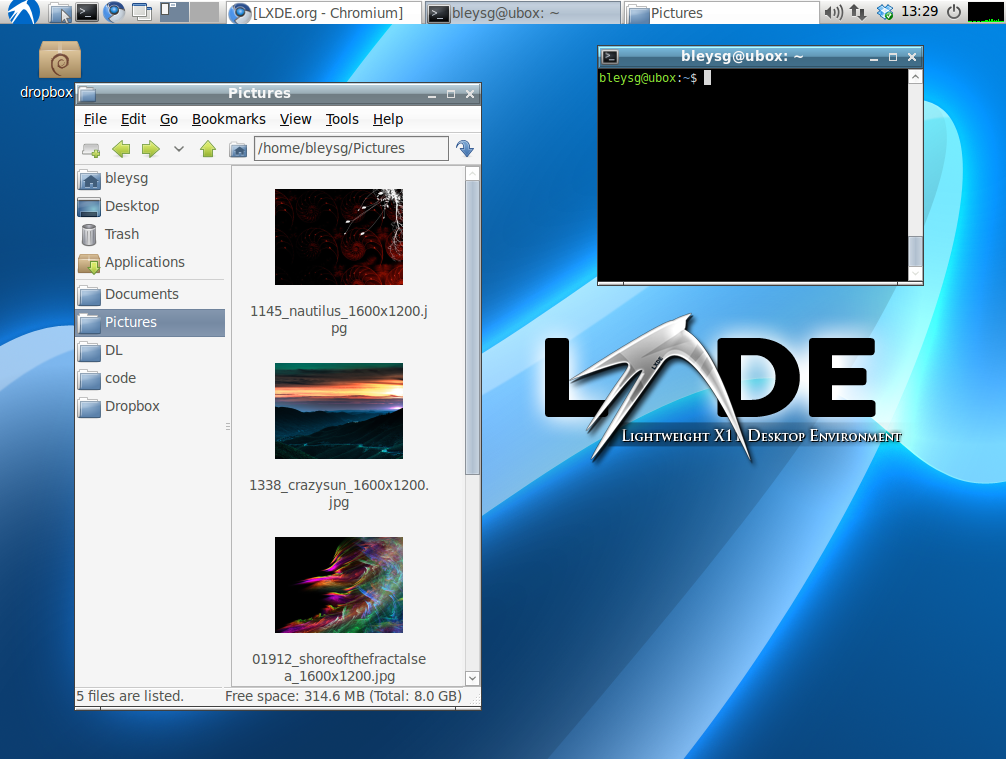
\includegraphics[width=250pt]{chapters/ch-brief-introduction-to-linux/figures/lxde_demo.png}
	\caption{LXDE desktop environment.} \label{ch:bitl:fig:lxdedemo}
\end{figure}

\begin{figure}
	\centering
	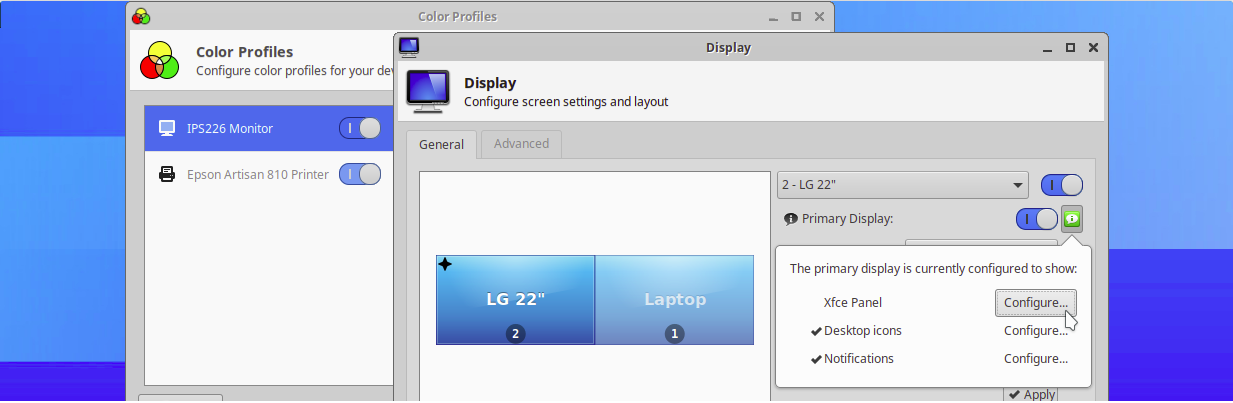
\includegraphics[width=250pt]{chapters/ch-brief-introduction-to-linux/figures/xfce_demo.png}
	\caption{Xfce desktop environment.} \label{ch:bitl:fig:xfcedemo}
\end{figure}

It is possible to install multiple desktop environment in one computer. In such a case, the user can choose which desktop environment to use each time the computer is powered on.

\section{Linux Installation}

Linux can be installed on a local PC hard disk, or on a mobile device such as a thumb drive. The installation of different distributions may differ. Thanks to the graphical installation tools for the popular distributions, the installations can be done easily by just following the instructions on the associated official sites.

Instructions of installing Ubuntu is given by \textit{https://ubuntu.com}. Instructions of installing Fedora is given by \textit{https://getfedora.org}. For the use of RHEL, consult with Red Hat at \textit{https://www.redhat.com}. Red Hat provides different types of RHEL licenses for different using purpose, including licenses for developers for developing individual APPs or training, which is cheaper than a standard enterprise-level license.
